\documentclass[a4paper,11pt]{article}

\usepackage[portuguese]{babel}
\usepackage[utf8]{inputenc}
\usepackage{amsmath}
\usepackage{graphicx}
\usepackage{hyperref}
\usepackage{float}
\usepackage{subfig}
\usepackage{fixltx2e}
\usepackage[bottom]{footmisc}
\usepackage{listings}
\usepackage{xargs}                      % Use more than one optional parameter in a new commands
\usepackage[pdftex,dvipsnames]{xcolor}  % Coloured text etc.
\usepackage[colorinlistoftodos,prependcaption,textsize=tiny]{todonotes}
\newcommandx{\unsure}[2][1=]{\todo[linecolor=red,backgroundcolor=red!25,bordercolor=red,#1]{#2}}
\newcommandx{\change}[2][1=]{\todo[linecolor=blue,backgroundcolor=blue!25,bordercolor=blue,#1]{#2}}
\newcommandx{\info}[2][1=]{\todo[linecolor=OliveGreen,backgroundcolor=OliveGreen!25,bordercolor=OliveGreen,#1]{#2}}
\newcommandx{\improvement}[2][1=]{\todo[linecolor=Plum,backgroundcolor=Plum!25,bordercolor=Plum,#1]{#2}}
\newcommandx{\thiswillnotshow}[2][1=]{\todo[disable,#1]{#2}}
\usepackage[font=footnotesize]{caption}
\usepackage[hypcap]{caption}
\usepackage[top=2.5cm, bottom=2.5cm, left=2.5cm, right=2.5cm]{geometry}
\usepackage{enumerate}
%\usepackage[siunitx,american]{circuitikz}

\setcounter{tocdepth}{3}
\setcounter{secnumdepth}{4}

\numberwithin{equation}{section}
\addto\captionsportuguese{\renewcommand{\contentsname}{Índice}}

\linespread{1.3}
\usepackage{indentfirst}

\begin{document}
\begin{titlepage}
\begin{center}

\hfill \break
\hfill \break


\includegraphics[width=0.3\textwidth]{img/logo}~\\[1cm] 

\textsc{\LARGE Instituto Superior Técnico}\\[0.25cm]
\textsc{\Large Mestrado Integrado em Engenharia Electrotécnica e de Computadores}\\[1.8cm]
\textsc{\huge Electrónica de Potência}\\[0.25cm]

\vspace{6mm}

{\huge \bfseries Conversor CA/CC Monofásico \linebreak Comandado de Meia Onda \\[0.7cm]}
{\bfseries Rectificador de meia onda com carga R e RL \& com carga RL e díodo de roda \\[1cm]}

\begin{tabular}{ l l }
	João Bernardo Sequeira de Sá & \hspace{2mm} n.º 68254 \\
	Maria Margarida Dias dos Reis & \hspace{2mm} n.º 73099 \\
	Rafael Augusto Maleno Charrama Gonçalves & \hspace{2mm} n.º 73786 \\
	Nuno Miguel Rodrigues Machado & \hspace{2mm} n.º 74236
\end{tabular}

\vspace{7mm}

Turno de Segunda-feira das 17h00 - 20h00

\vfill

{\large Lisboa,  de Novembro de 2015} 
	
\end{center}
\end{titlepage}
	
\tableofcontents
\pagebreak

\section{Introdução}

Com este trabalho pretende estudar-se o funcionamento do conversor CA/CC (Retificador) monofásico comandado de meia onda.

Este tipo de retificadores tira o seu nome da capacidade que o Tiristor tem em controlar a sua tensão de saída através do ângulo de disparo. O Tiristor é levado à condução pela aplicação de um sinal na \textit{Gate} e passa ao corte através de comutação natural na maioria dos casos, ou comutação forçada no caso de circuitos fortemente indutivos. \cite{Rashid}

Pode dizer-se que este trabalho está dividido em duas partes. Na primeira estuda-se o retificador de meia onda simples com carga R e RL. Na segunda parte trata-se da inclusão de um díodo de roda livre e estuda-se o comportamento deste novo circuito de potência com uma carga RL.

O comportamento do Retificador de meia onda com uma carga resistiva pura é tal que a corrente e a tensão na carga têm que apresentar a mesma polaridade em qualquer altura. Devido ao comportamento do Tiristor apenas existe tensão na saída durante alternâncias positivas, pois quando a corrente se anula no Tiristor este passa ao corte, sendo esta característica do comportamento que leva ao nome "de meia onda". \cite{Kassakian}

Já no caso de uma carga RL existe uma ligeira desfasagem entre tensão e corrente, devido à presença da bobine, pelo que a corrente no Tiristor apenas se anula quando a tensão já se encontra na sua alternância negativa. Embora continuemos a ter apenas meia onda, já não existe uma distinção certa entre conduzir apenas durante uma das alternâncias. \cite{Kassakian}

Na segunda parte deste trabalho inclui-se ao circuito um Díodo de Roda Livre. O Díodo de Roda Livre é também conhecido como Díodo \textit{Snubber} ou Díodo \textit{Flyback} \cite{Silva}. Este é utilizado para prevenir valores negativos de tensão na saída assim como eliminar os picos de tensão quando se têm cargas indutivas a sofrer comutação. \cite{Kassakian}



\section{Condução do Trabalho}

\subsection{Estudo do circuito de disparo}

O circuito de disparo utilizado neste trabalho pode ser representado por um diagrama de blocos tal como se observa na \autoref{fig:circuit_1}.

Como este está preparado para servir como circuito de disparo para um Retificador de Ponte Completa, inclui a capacidade para realizar o \textit{Trigger} de 4 Tiristores, sendo estes disparados aos pares e consecutivamente. O circuito é constituído por um transformador que amostra a tensão de entrada (TR\_SINC), garantindo a sincronia entre a geração dos impulsos e a tensão; um circuito integrado (UAA145), que detecta a passagem da tensão da rede por zero e gera impulsos em $\alpha$ e $\alpha + \pi$ e um circuito integrado (NE555) e duas portas lógicas $NAND$, que combinam os impulsos num trem e garantem que a potência da \textit{Gate} dos Tiristores não é excedida.

\begin{figure}[h]
	\centering
	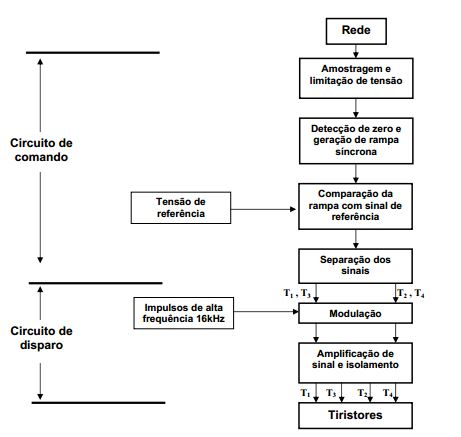
\includegraphics[keepaspectratio=true, scale=0.8]{teoricas/circuito_disparo.jpg}
	\caption{Diagrama de blocos do Circuito de Disparo.}
	\label{fig:circuit_1}
	\vspace{-0.8em}
\end{figure}

\subsubsection{Formas de onda dos sinais de disparo}

Para que fosse possível estudar o funcionamento do circuito de disparo começou por se observar as formas de onda da tensão amostrada de entrada e dos impulsos gerados.

\begin{figure}[h]
	\centering
	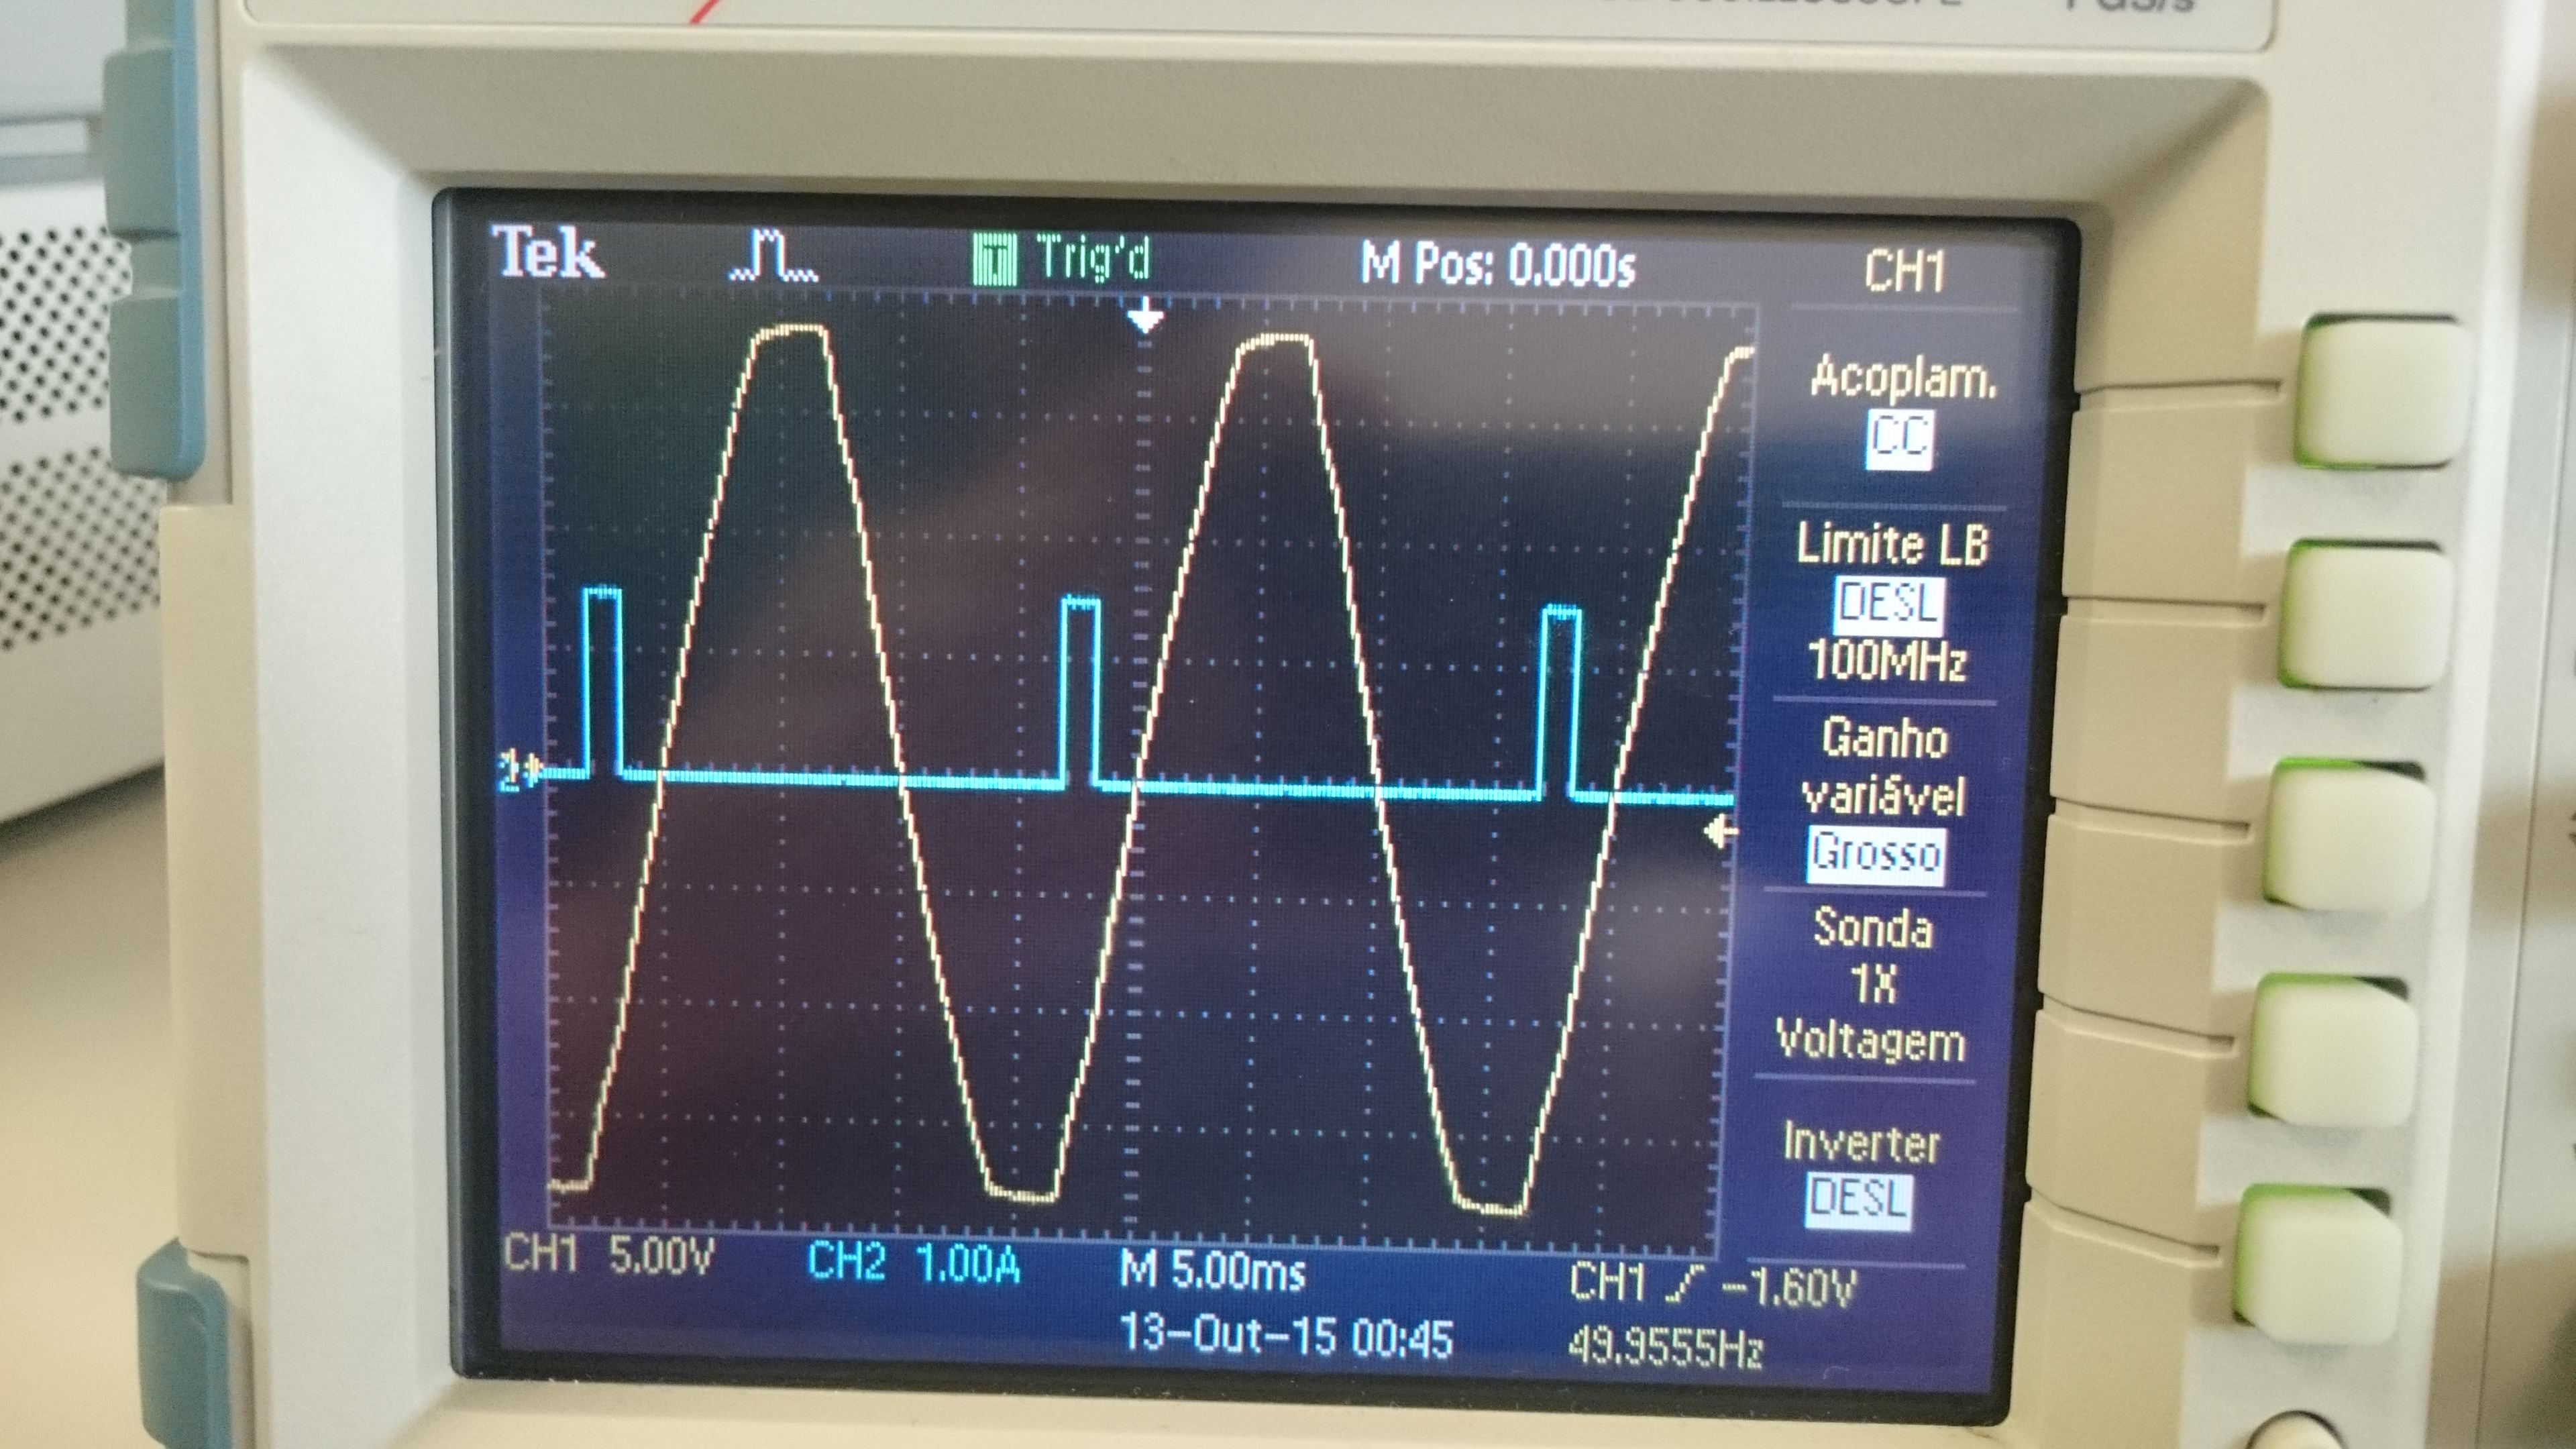
\includegraphics[keepaspectratio=true, scale=0.11]{img/figs/AB_1.jpg}
	\caption{Forma de onda da tensão em A e B.}
	\label{fig:AB_1}
	\vspace{-0.8em}
\end{figure}

\begin{figure}[h]
	\centering
	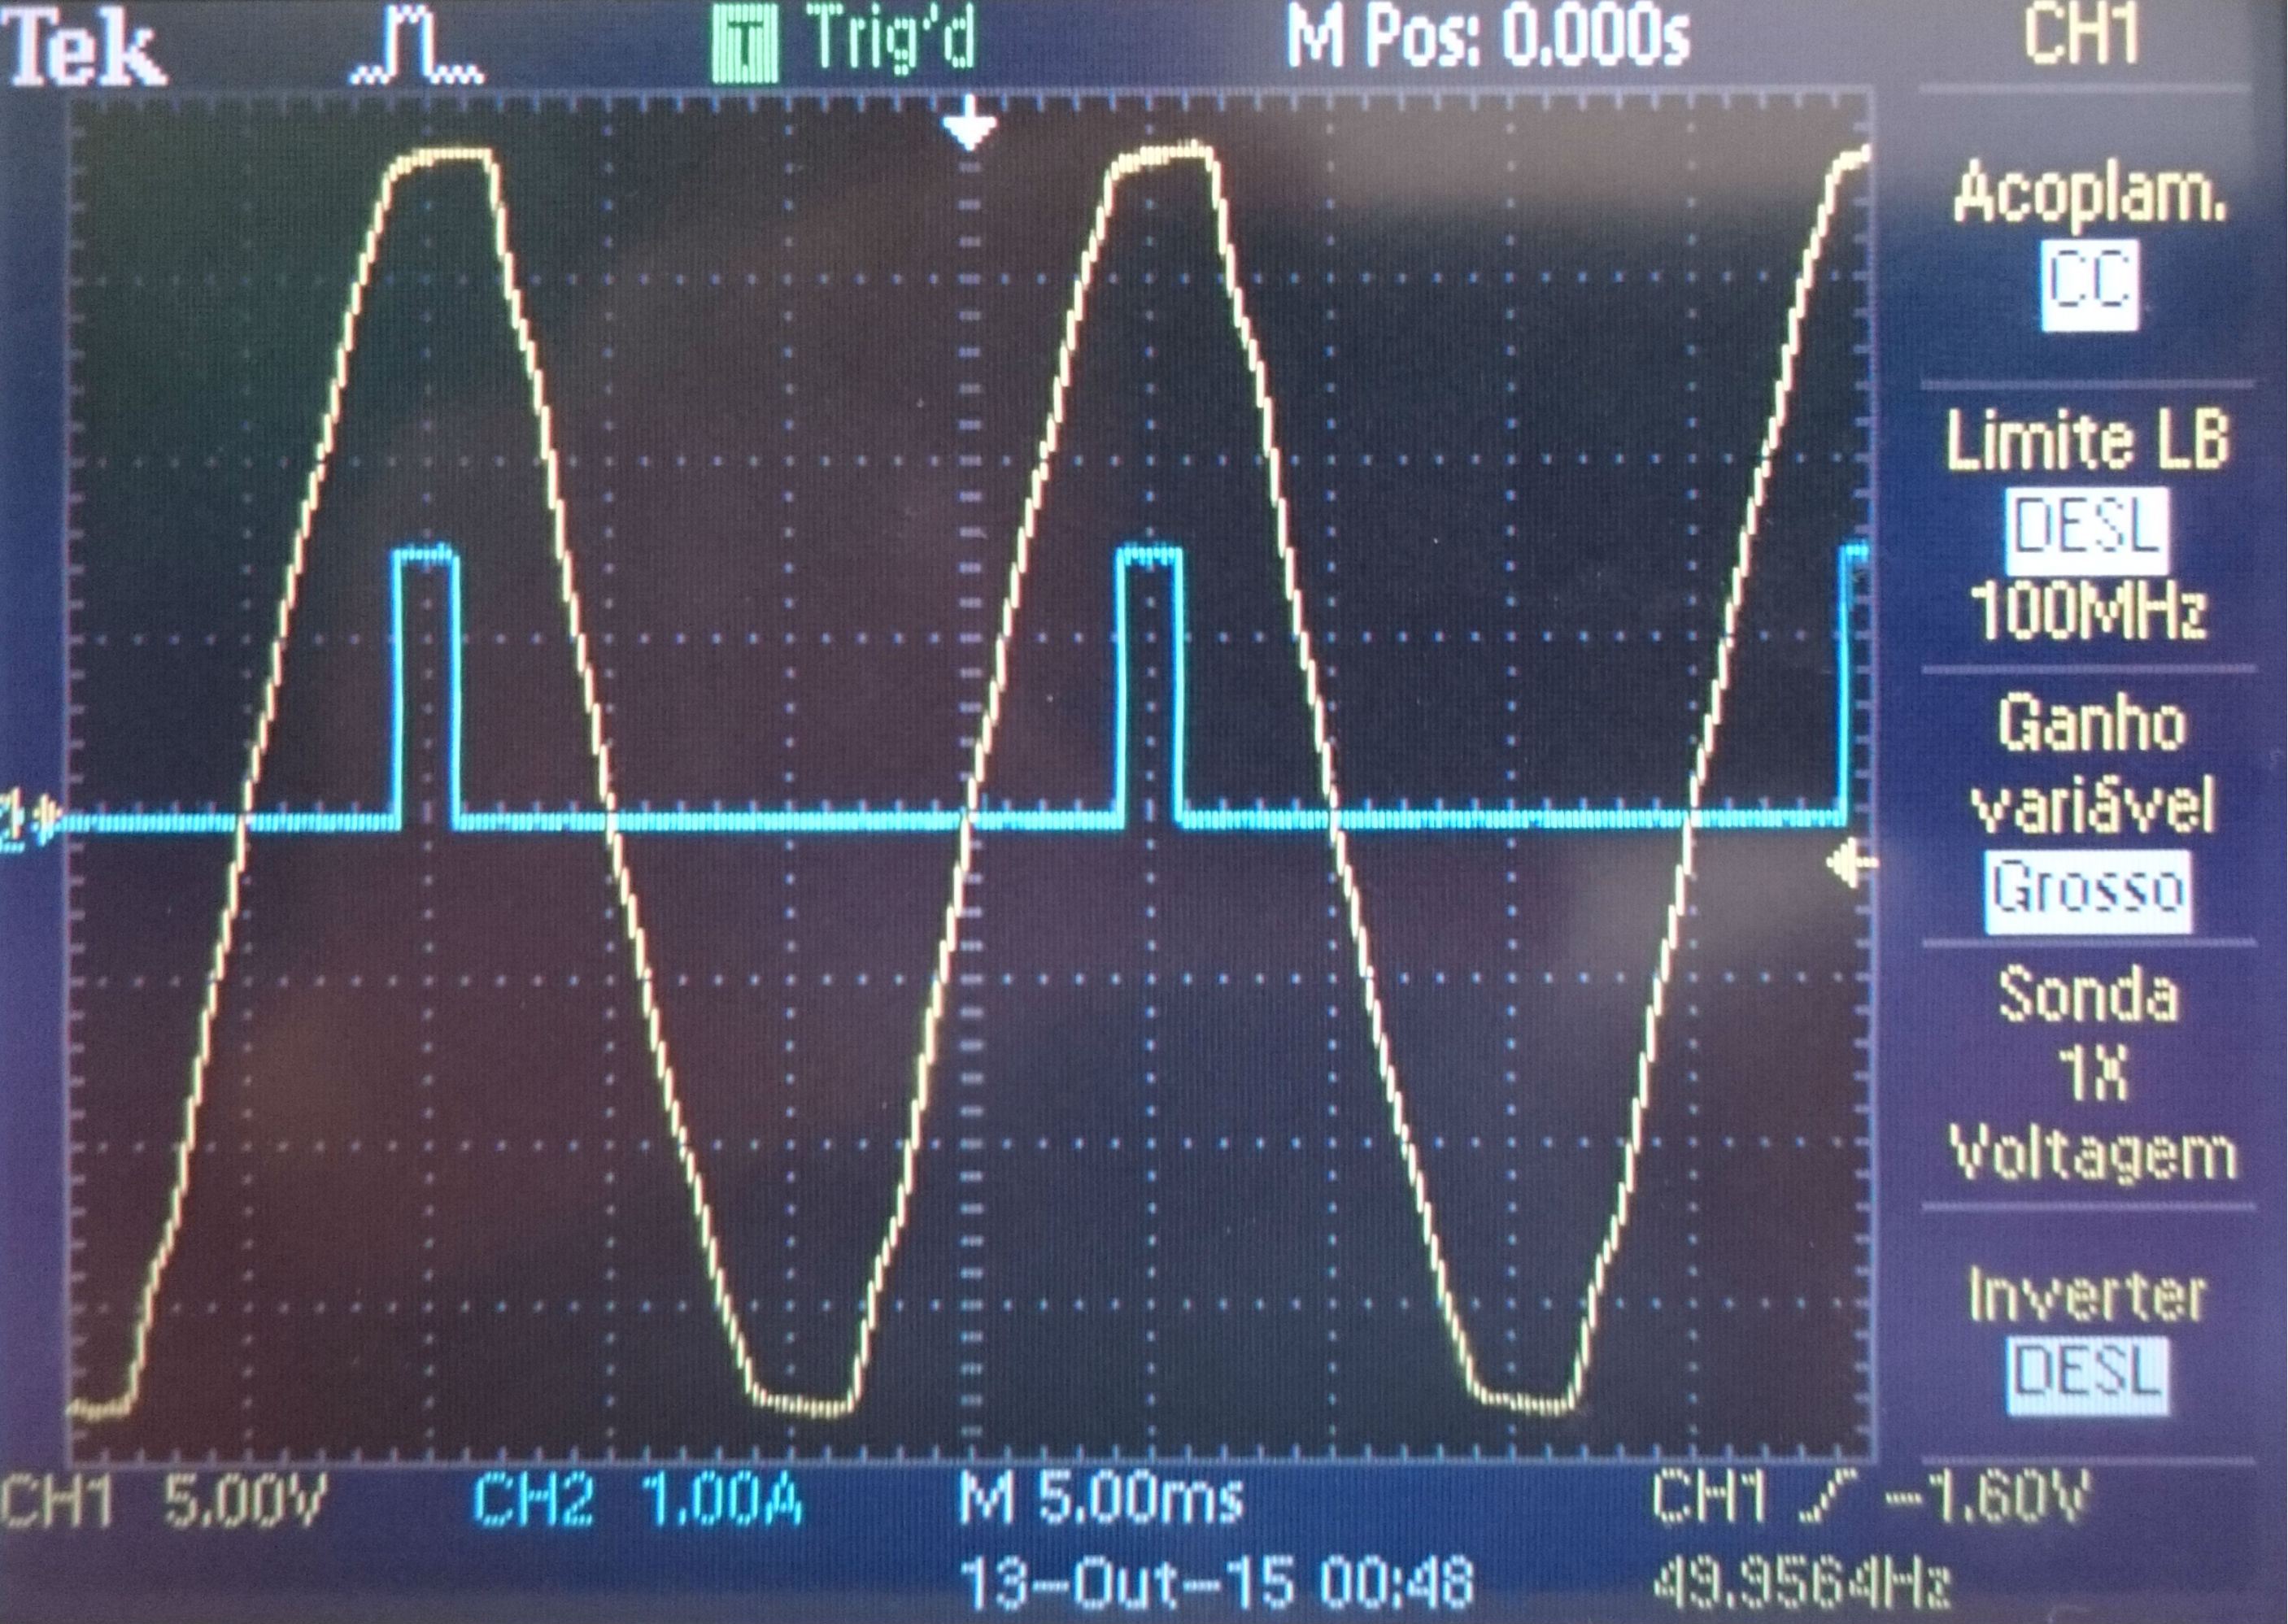
\includegraphics[keepaspectratio=true, scale=0.1]{img/figs/AC_1.jpg}
	\caption{Forma de onda da tensão em A e C.}
	\label{fig:AC_1}
	\vspace{-0.8em}
\end{figure}

Na \autoref{fig:AB_1} pode ver-se a amarelo a tensão amostrada pelo transformador e a azul o impulso de \textit{Trigger} gerado para $\alpha$. Já na \autoref{fig:AC_1} pode observar-se a amarelo novamente a tensão amostrada e a azul o impulso de \textit{Trigger} gerado para $\alpha + \pi$.

A posição destes dois impulsos pode ser controlada através do valor do ângulo de disparo $\alpha$ rodando um manipulo presente na placa do Circuito de Disparo. Ao mudar este valor, as formas de onda são observáveis, tanto para a tensão amostrada e o impulso $\alpha$ como para a mesma tensão e o impulso  $\alpha + \pi$, na \autoref{fig:AB_2} e \autoref{fig:AC_2} respectivamente.

\begin{figure}[h]
	\centering
	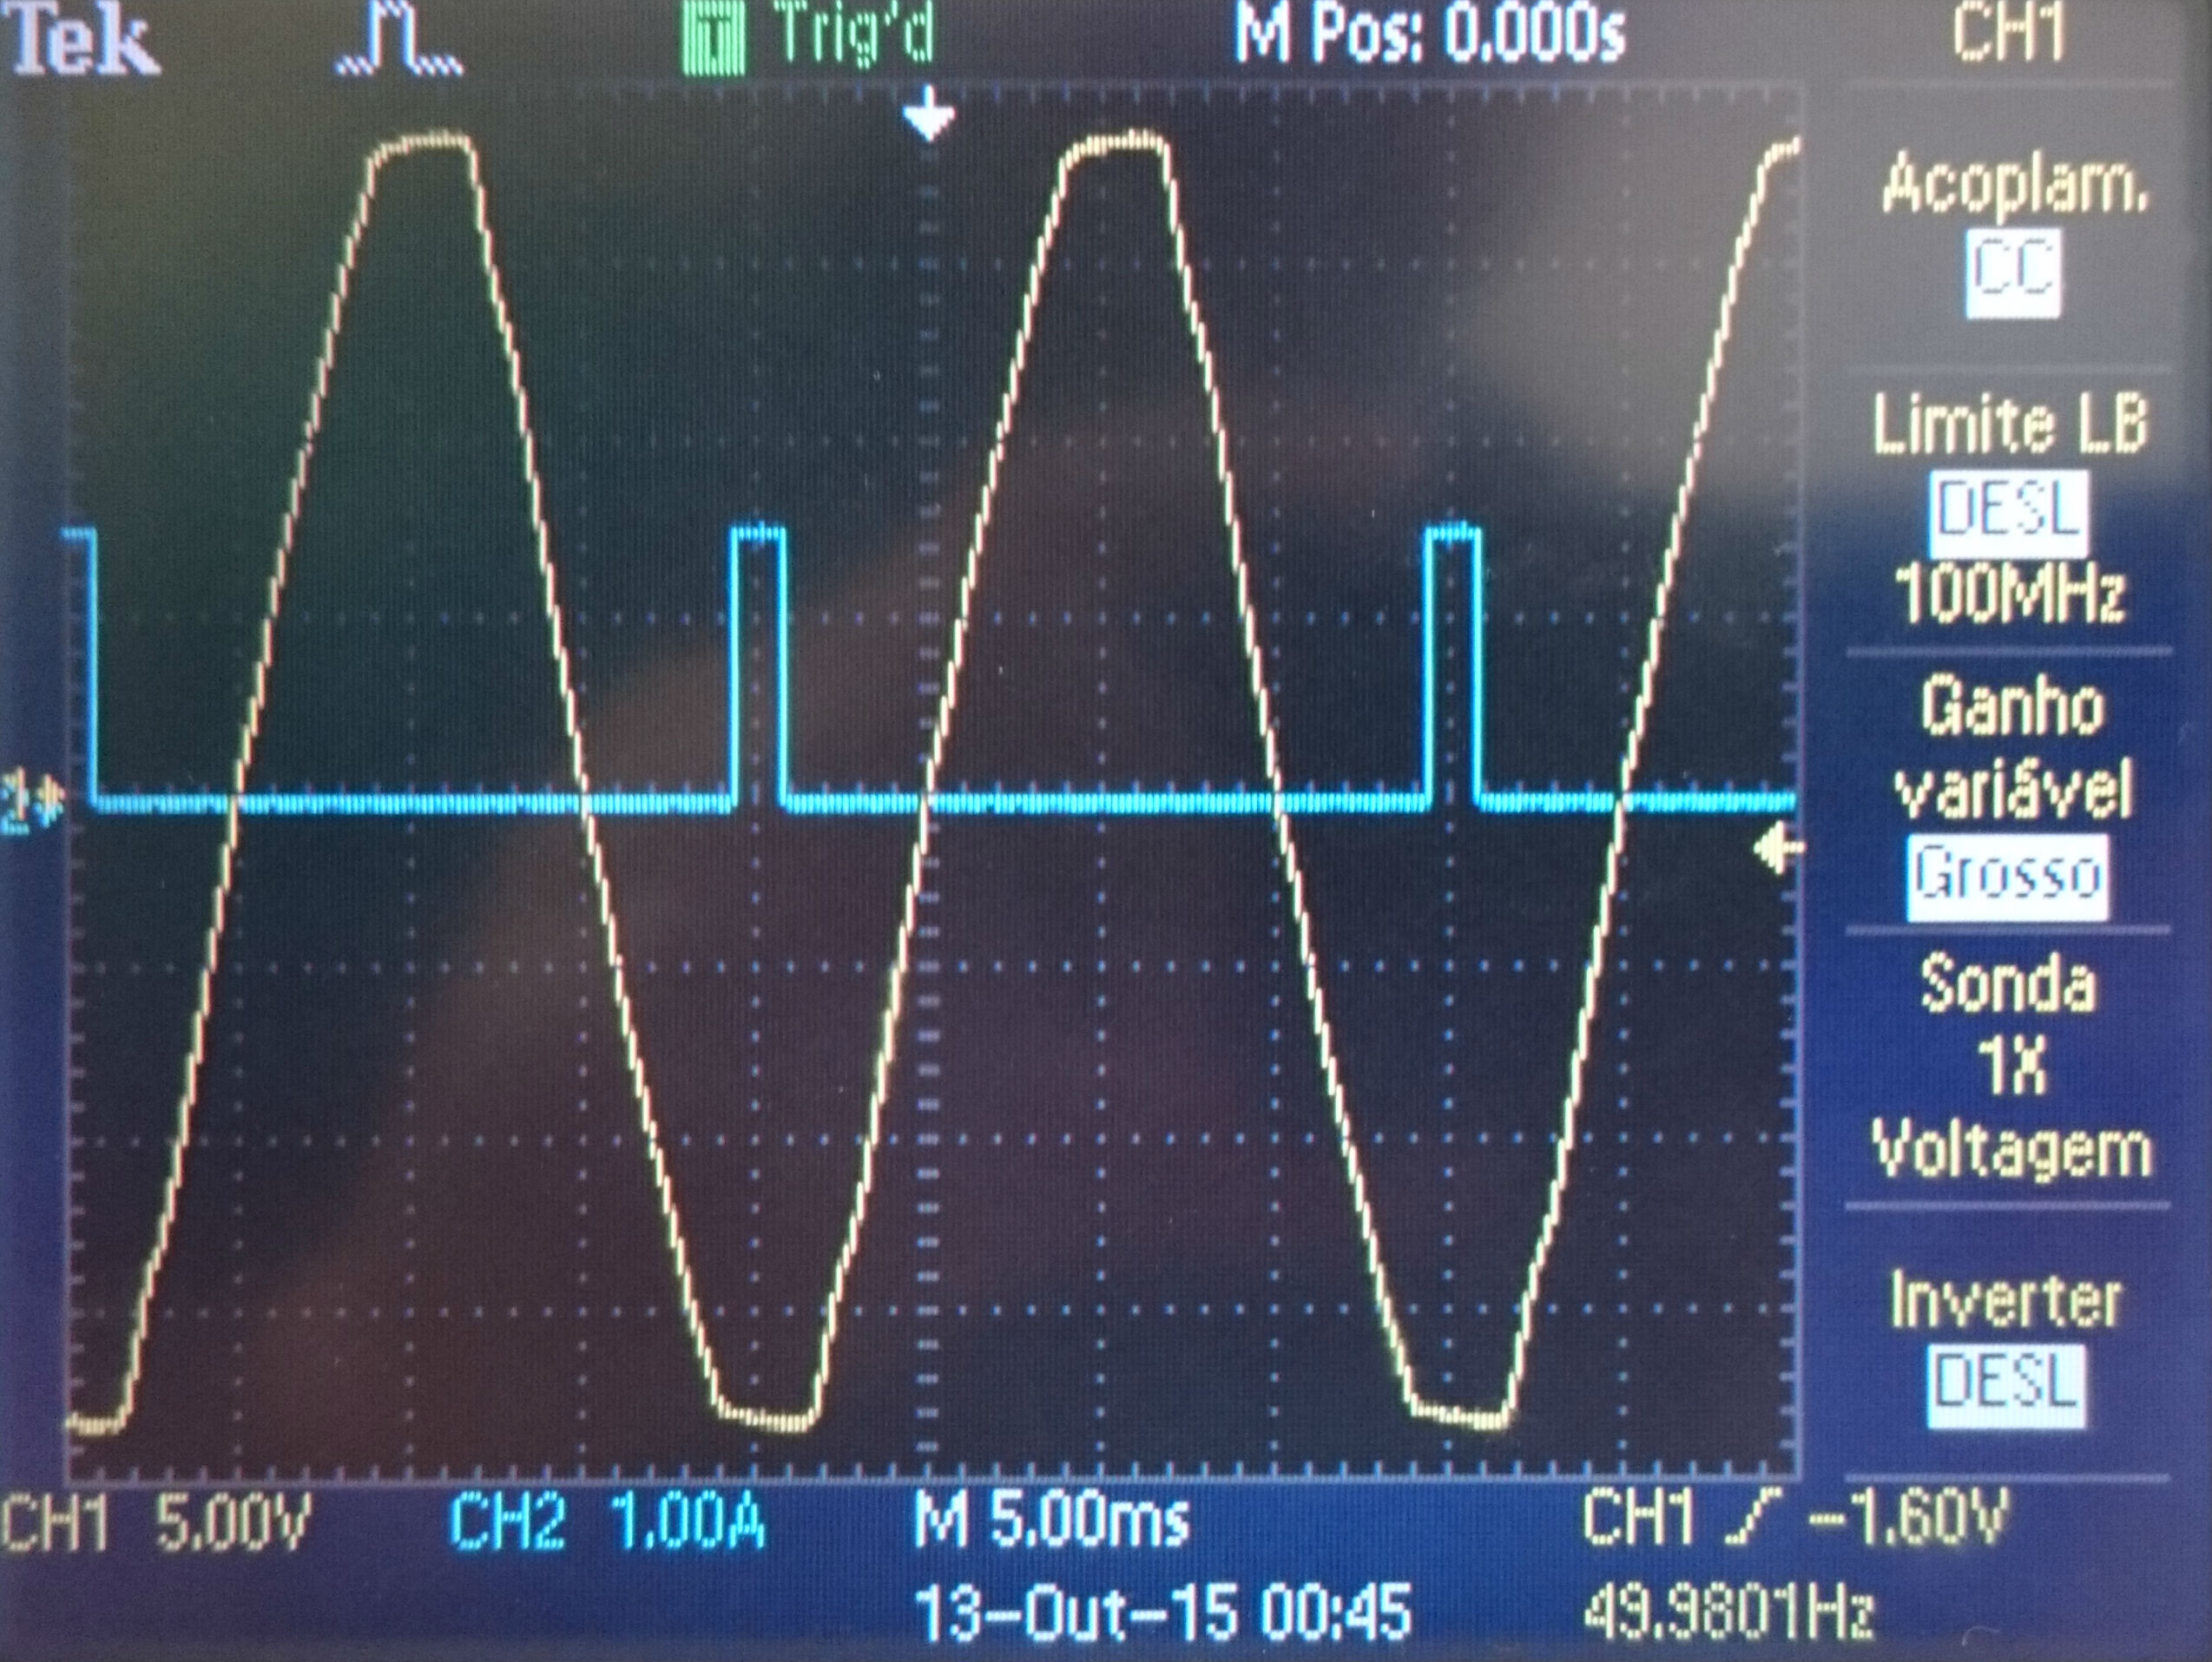
\includegraphics[keepaspectratio=true, scale=0.11]{img/figs/AB_2.jpg}
	\caption{Forma de onda da tensão em A e B para novo $\alpha$.}
	\label{fig:AB_2}
	\vspace{-0.8em}
\end{figure}

\begin{figure}[h]
	\centering
	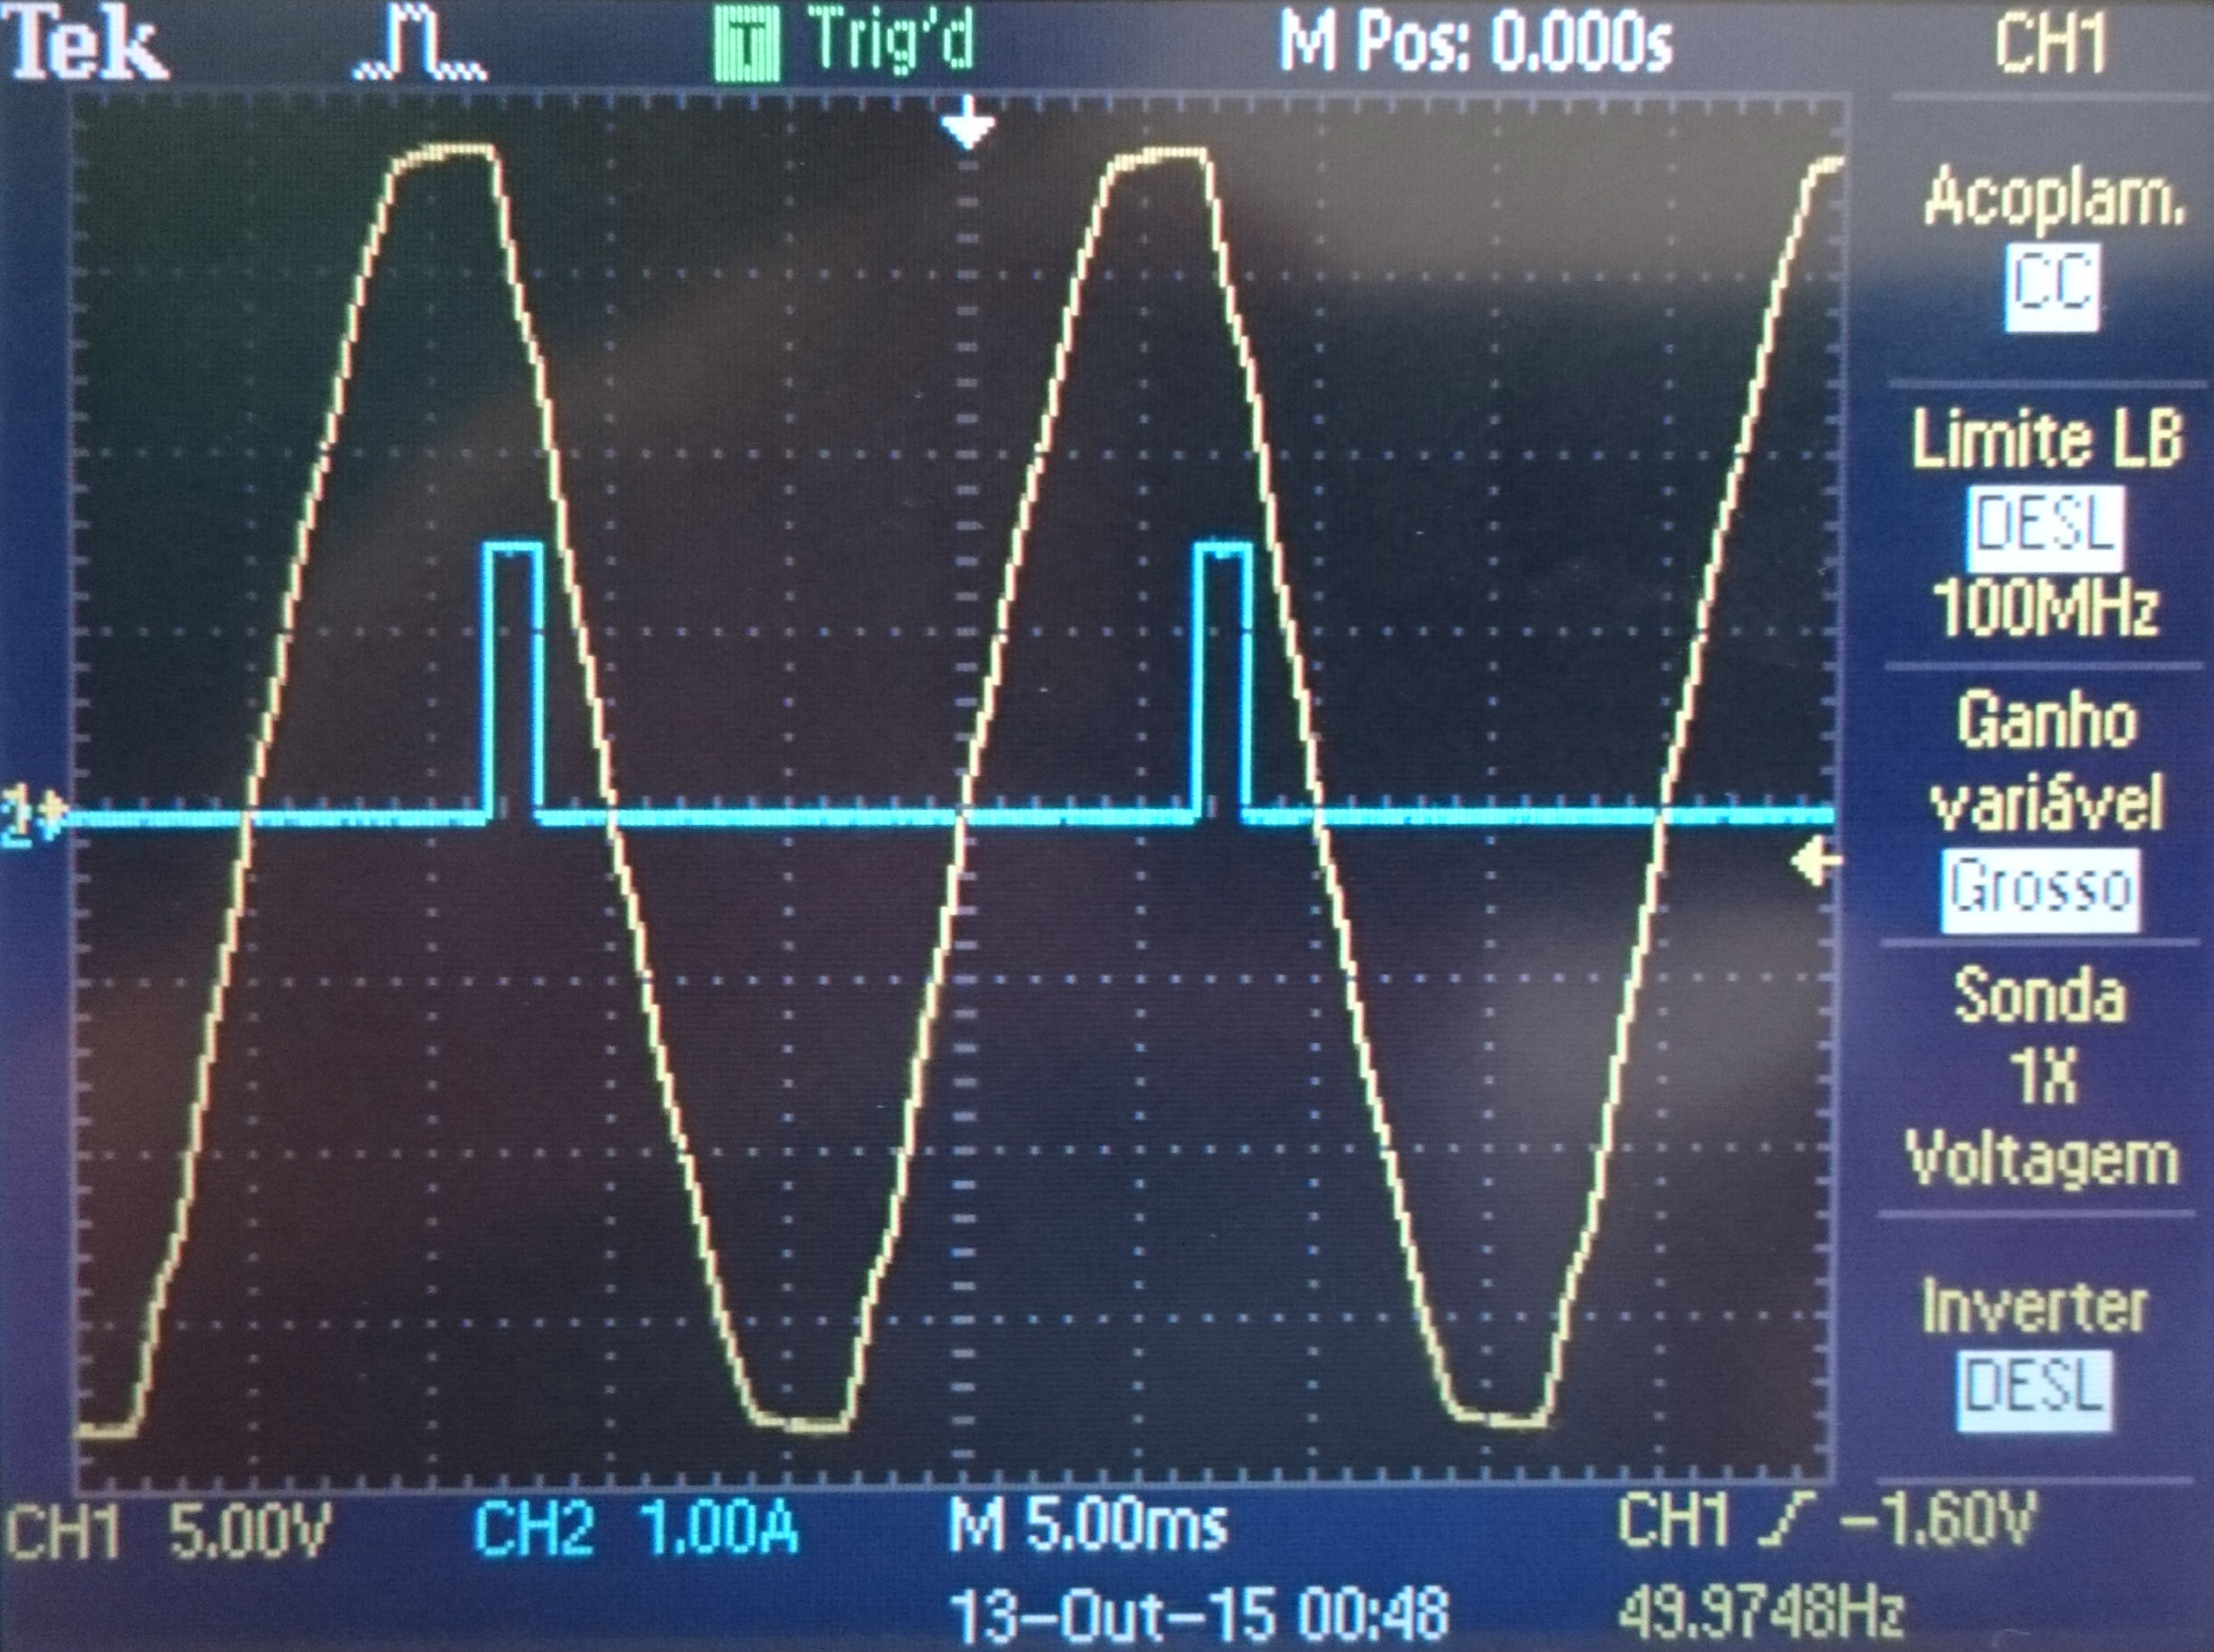
\includegraphics[keepaspectratio=true, scale=0.11]{img/figs/AC_2.jpg}
	\caption{Forma de onda da tensão em A e C para novo $\alpha$.}
	\label{fig:AC_2}
	\vspace{-0.8em}
\end{figure}


\subsubsection{Trem de impulsos}

Como a frequência de operação é a da rede, $50$ Hz, os impulsos de disparo devem ter durações de poucos milissegundos, evitando-se efeitos negativos de \textit{latching}, sendo estes especialmente prevalentes no caso de cargas indutivas em que o ângulo de disparo será elevado. No entanto estas durações podem saturar o transformador de impulsos ou provocar perdas elevadas na \textit{Gate} do Tiristor.

Para resolver ambos estes problemas utiliza-se um trem de impulsos de \textit{Trigger}.

\begin{figure}[h]
	\centering
	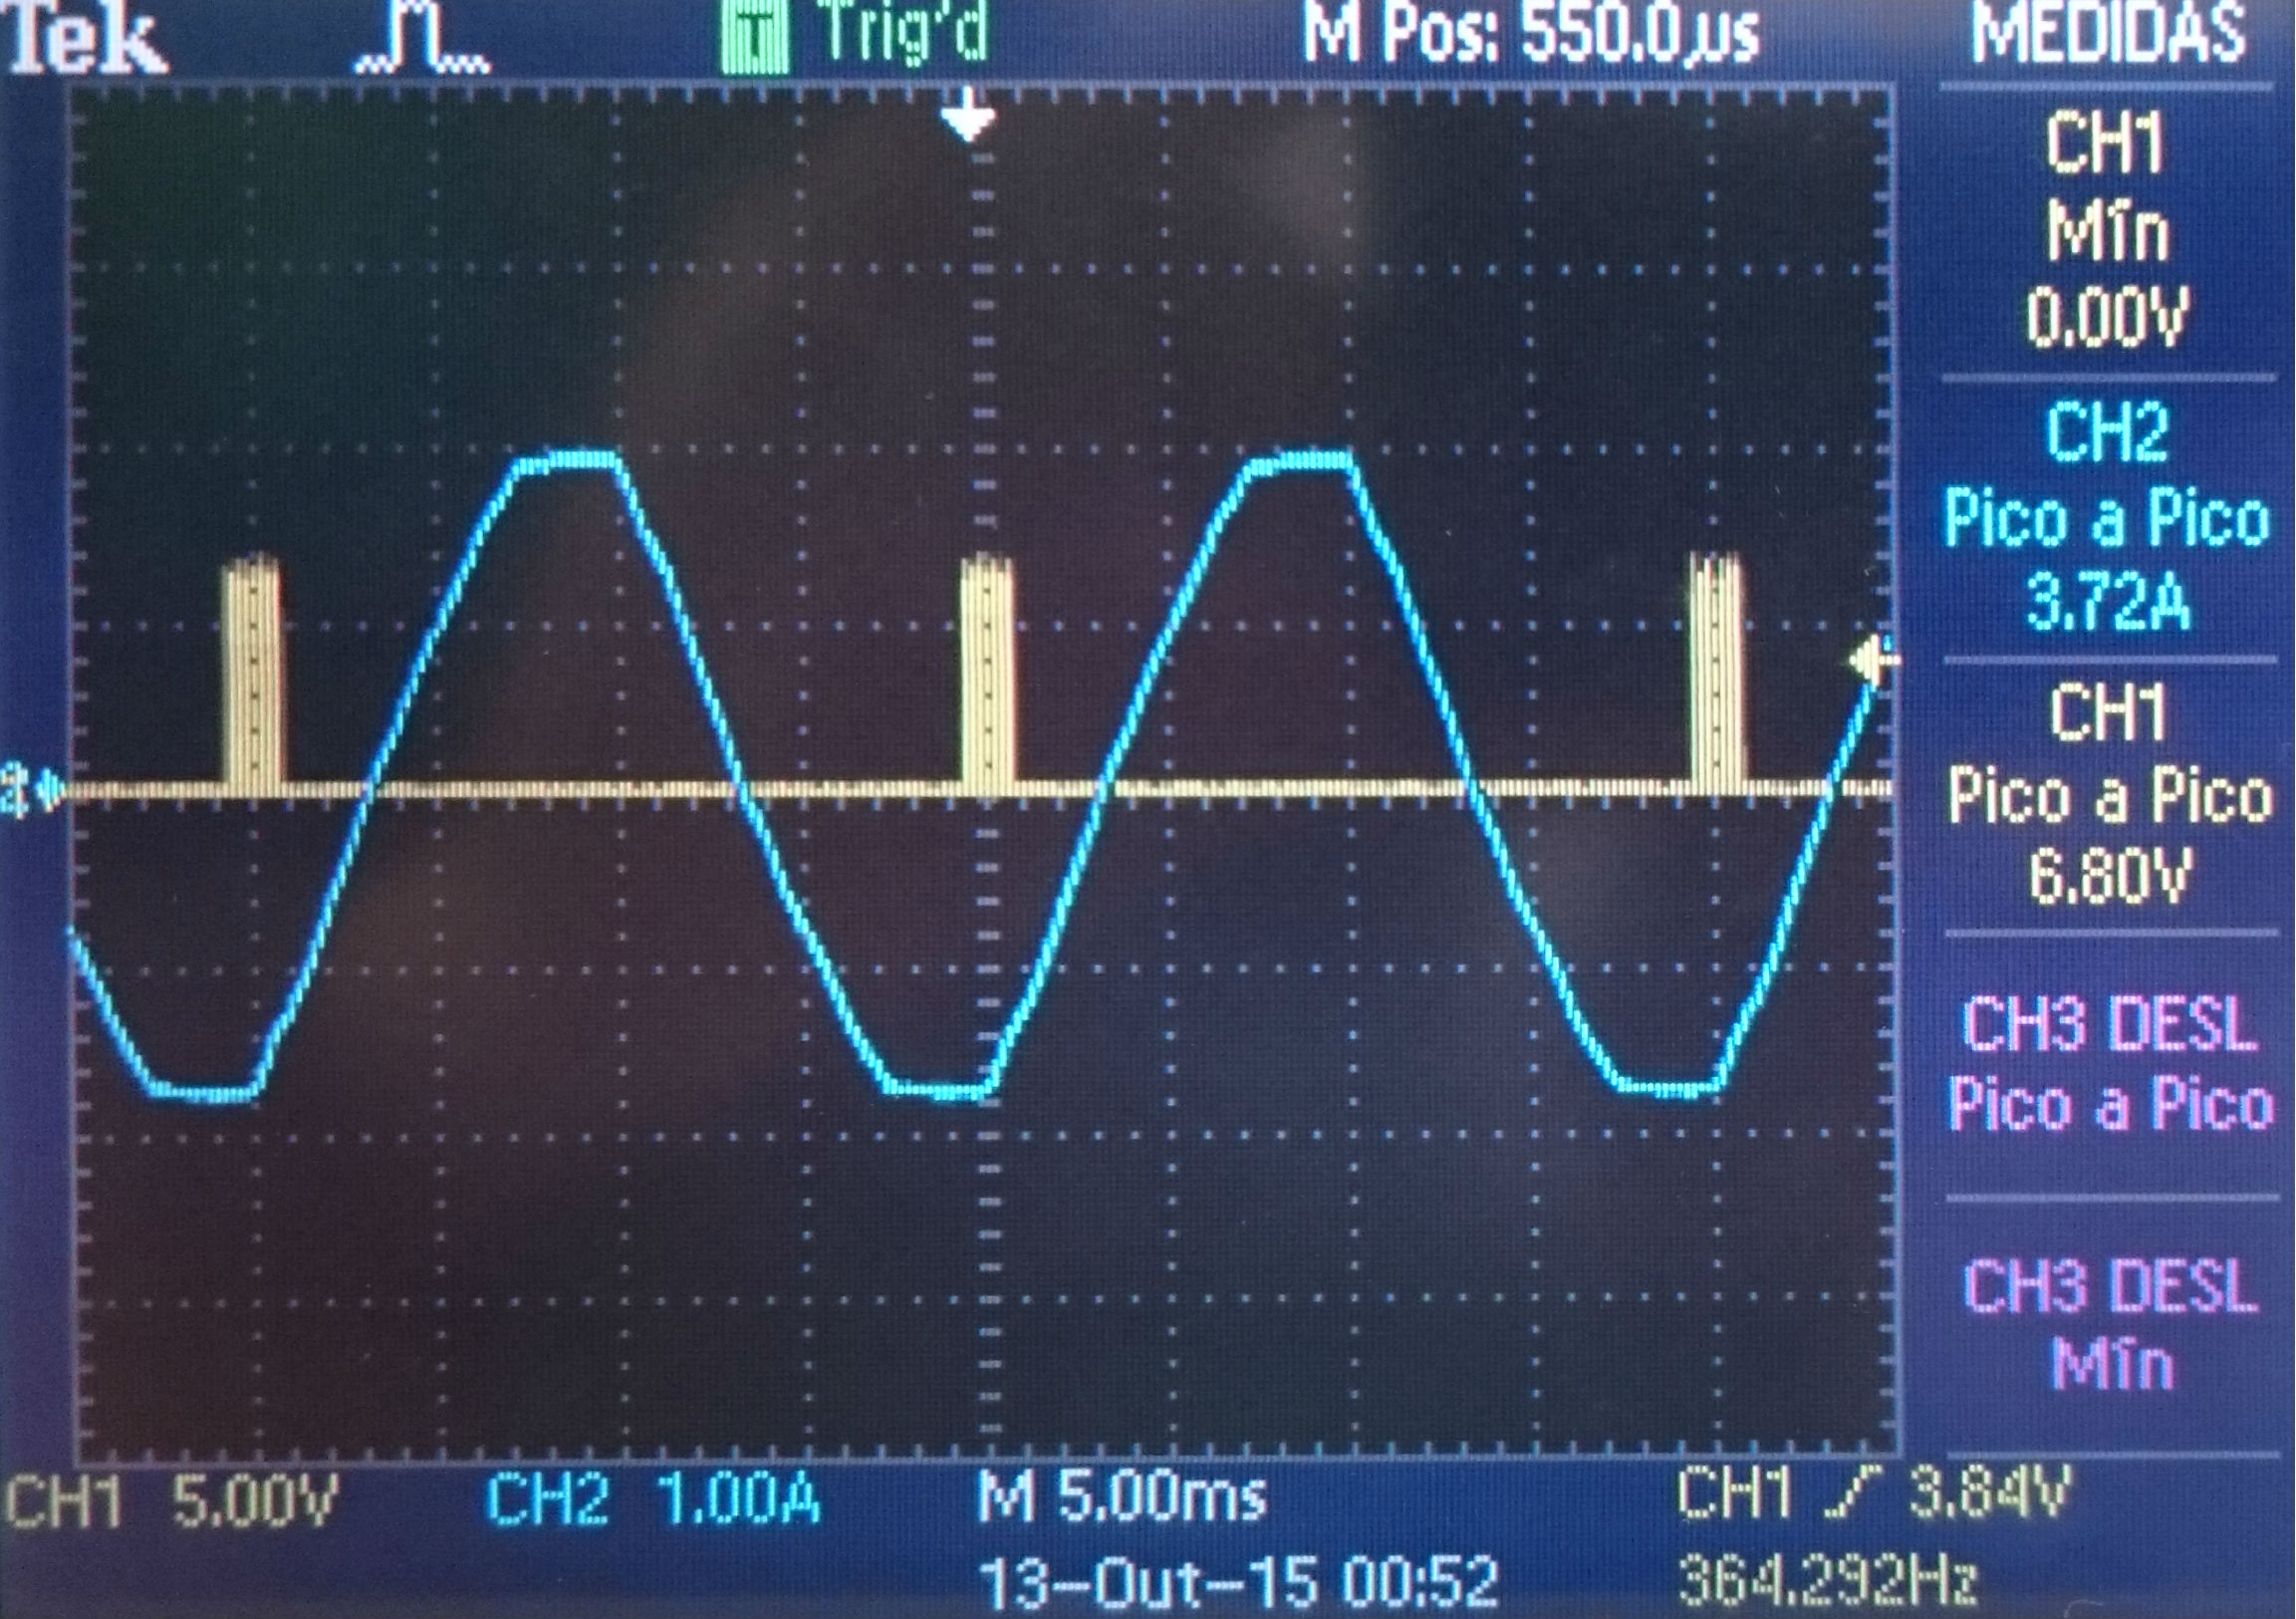
\includegraphics[keepaspectratio=true, scale=0.115]{img/figs/trem_impulsos_A.jpg}
	\caption{Formas de onda do trem de impulso e tensão em A.}
	\label{fig:trem_impulsos_A}
	\vspace{-0.8em}
\end{figure}

Colocou-se entre a \textit{Gate} e o Cátodo uma resistência de $33$ $\Omega$ para simular a \textit{Gate} do tiristor. Na \autoref{fig:trem_impulsos_A} pode assim ver-se a azul a queda de tensão nessa resistência e a amarelo o trem de impulsos.

\begin{figure}[h]
	\centering
	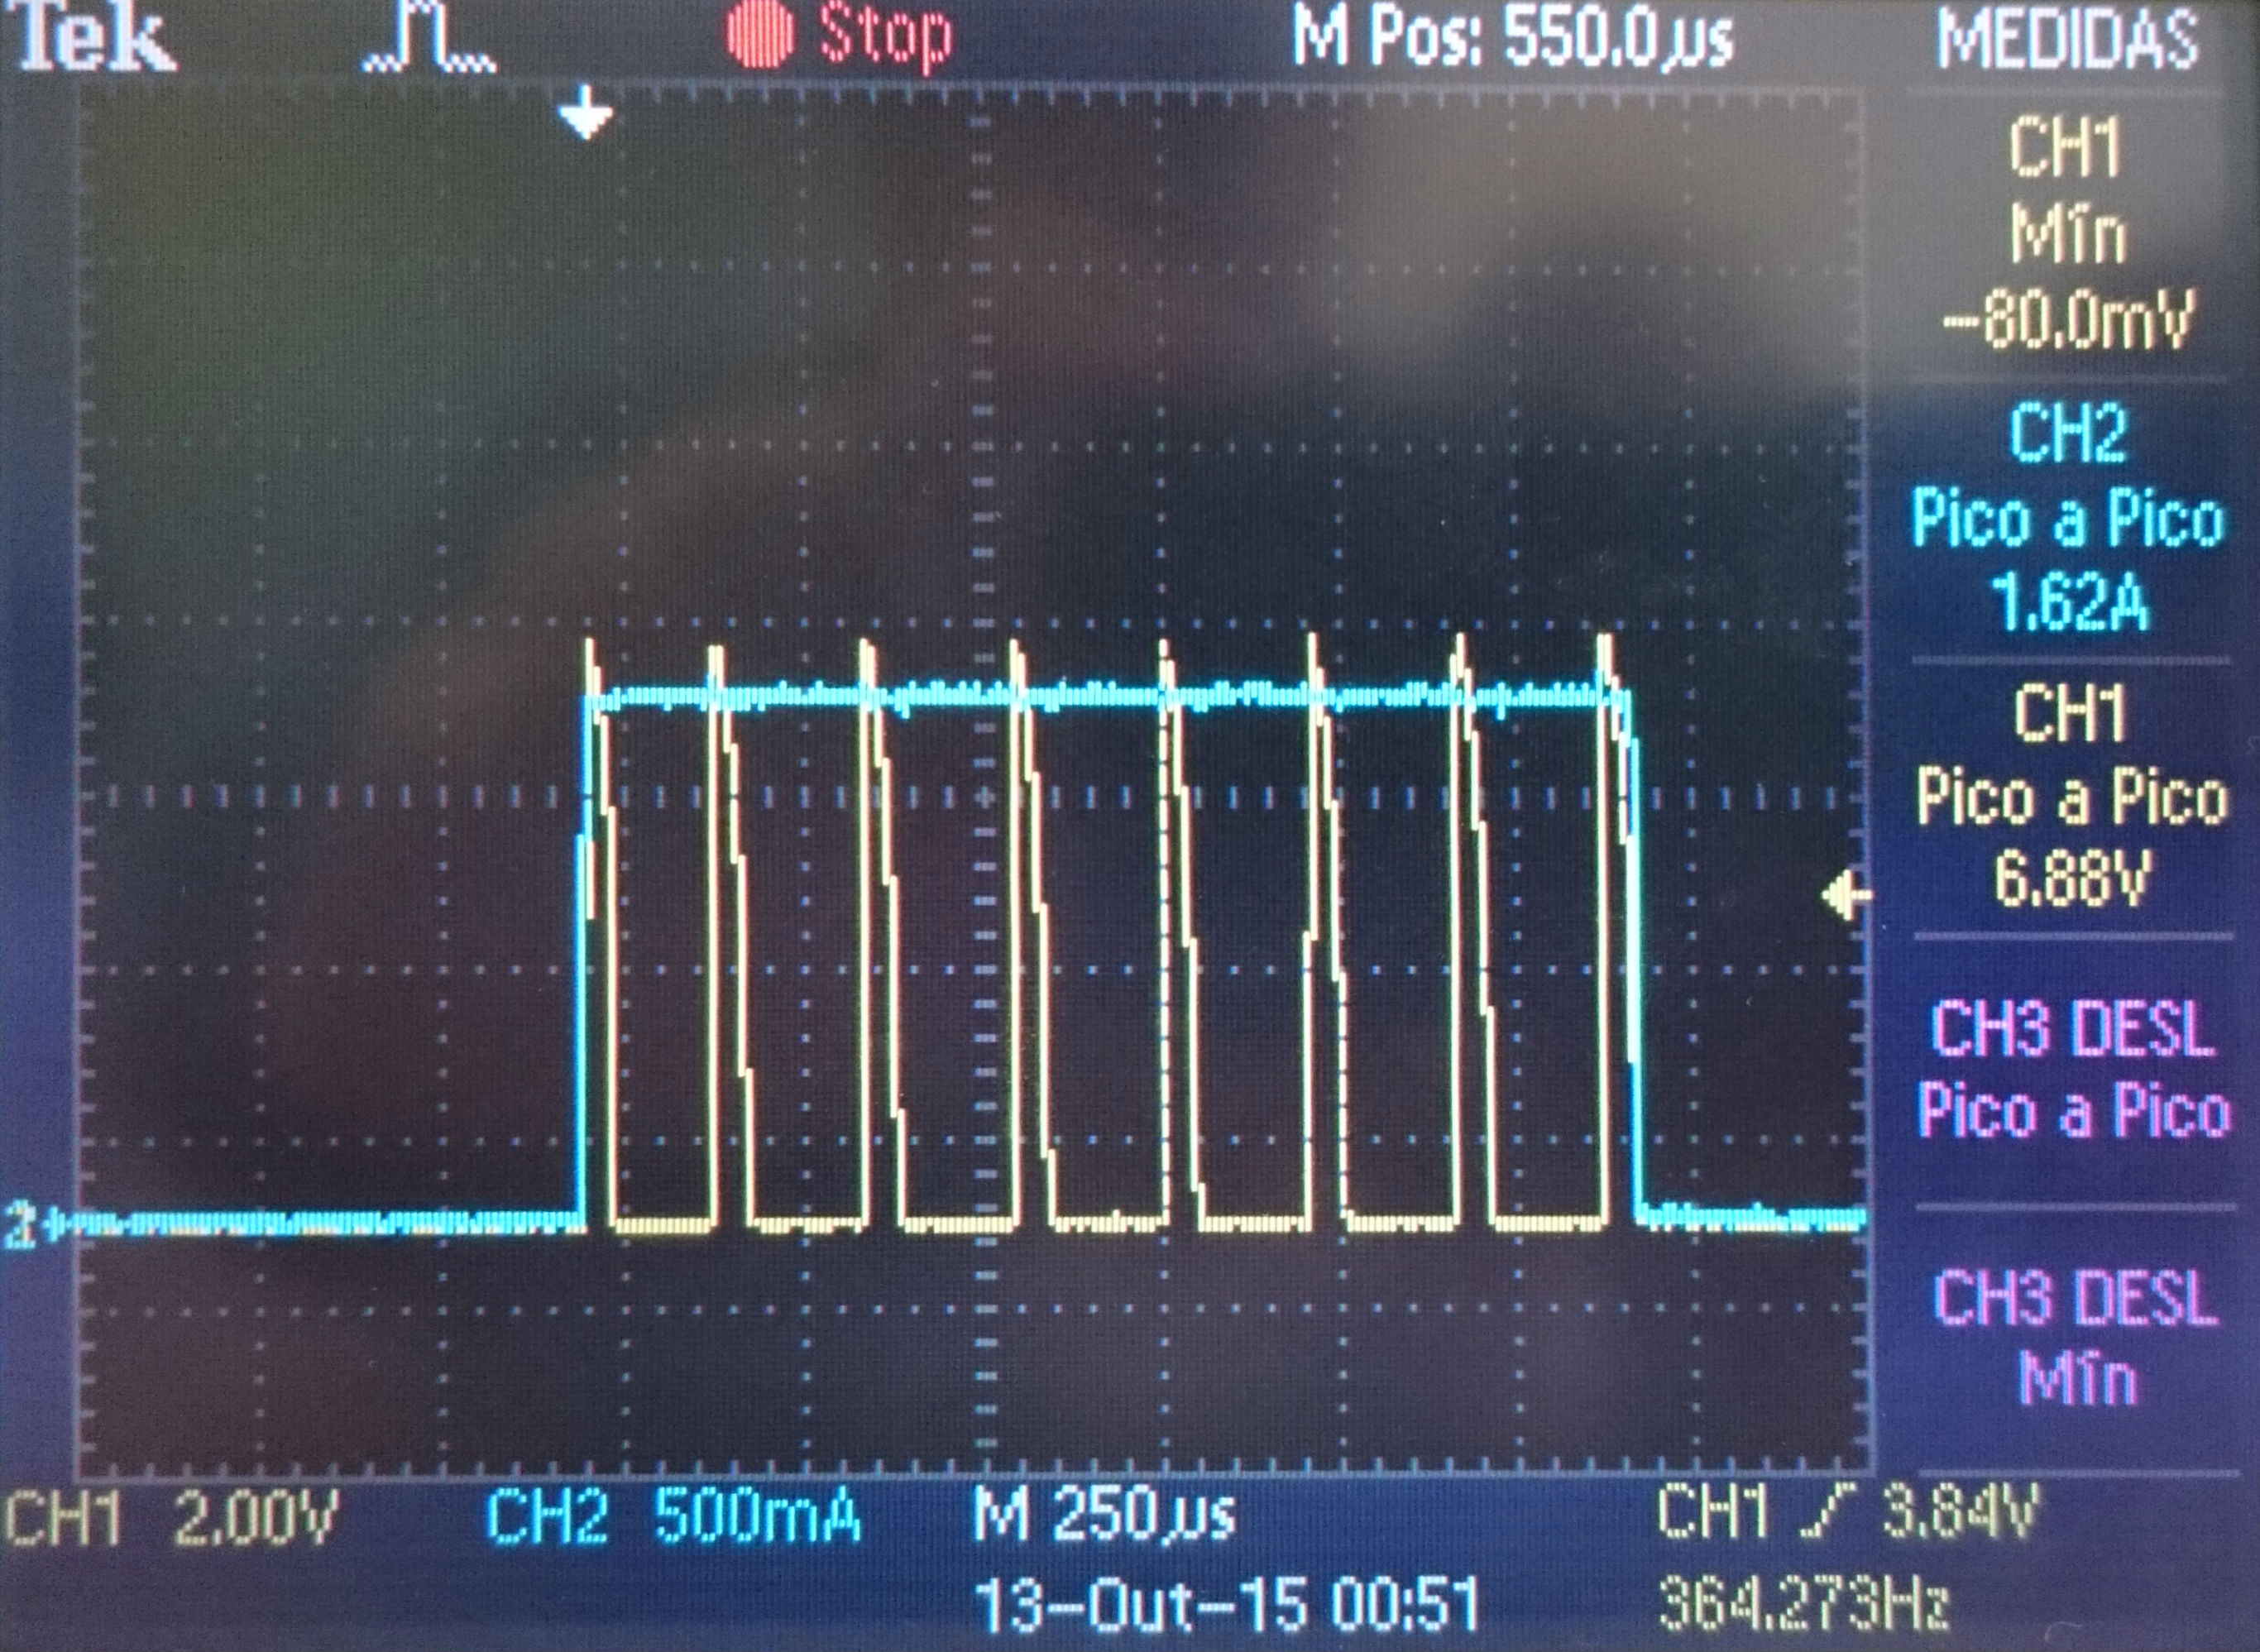
\includegraphics[keepaspectratio=true, scale=0.09]{img/figs/trem_impulsos_B.jpg}
	\caption{Formas de onda do trem de impulso e tensão em B.}
	\label{fig:trem_impulsos_B}
	\vspace{-0.8em}
\end{figure}

Na \autoref{fig:trem_impulsos_B} pode também observar-se o trem de impulsos, a amarelo, face ao impulso original correspondente, a azul.


\subsection{Estudo do circuito de potência}

\subsubsection{Carga resistiva pura (R)}

Para que se possa estudar o funcionamento do Retificador para cargas Resistivas puras utilizou-se um reóstato como carga, regulando-o para perto de meio ficando-se com cerca de $16$ $\Omega$.

\paragraph{Formas de onda da tensão e corrente na entrada}

\begin{figure}[h]
	\centering
	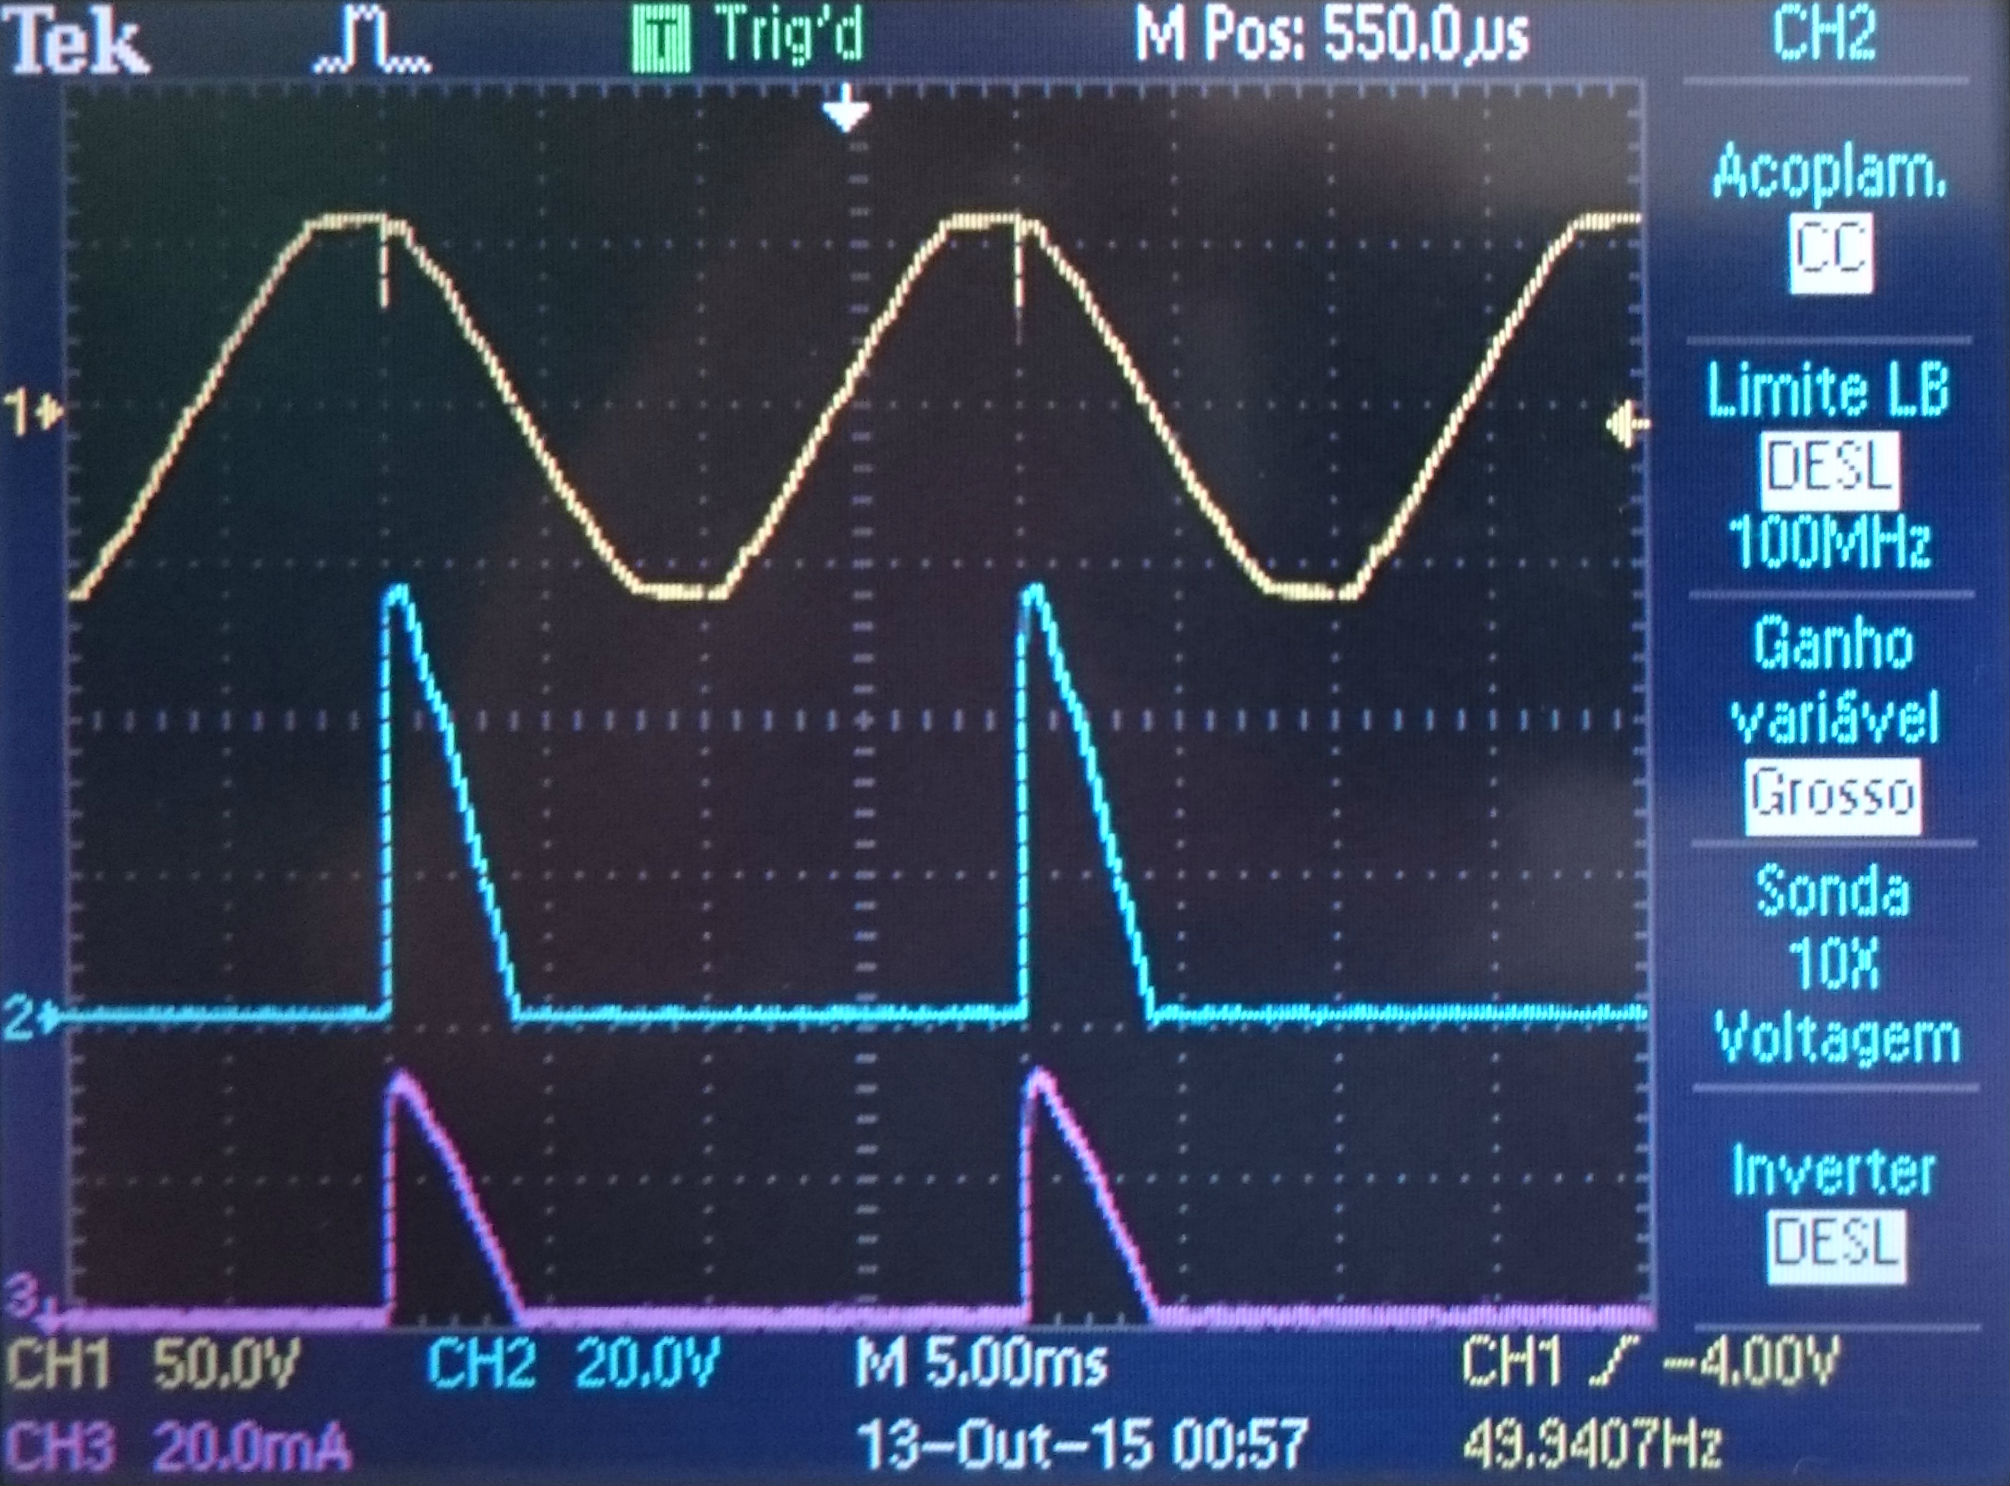
\includegraphics[keepaspectratio=true, scale=0.12]{img/figs/carga_resistiva.jpg}
	\caption{Formas da tensão na entrada e corrente e tensão na carga para carga R.}
	\label{fig:carga_resistiva}
	\vspace{-0.8em}
\end{figure}


Na \autoref{fig:carga_resistiva} observa-se o funcionamento do circuito quando sujeito uma carga resistiva pura. A tensão de entrada pode ser vista a amarelo estando a tensão e corrente na carga a azul e roxo respetivamente.

\paragraph{Formas de onda da tensão e corrente na saída}


\unsure{pode apagar-se esta secção porque a imagem ja foi mostrada na anterior}

\paragraph{Formas de onda da tensão e corrente no tiristor}

\unsure{não temos esta imagem. Podemos roubar a imagem do edson ou ser honestos, dizer que nos esquecemos de tirar a foto e por aqui uma imagem da simualação equivalente}

\paragraph{Valores médio e eficaz da tensão e corrente na carga}

Os valores médio e eficaz de tensão e corrente na carga podem ser obtidos através das seguintes expressões:

\[v_i(t)=A \sin(\omega t)\]

\[V_{oMED} (t) = \frac{1}{2\pi} \int_{\alpha}^{\pi} A \sin(\omega t) d \omega t = \frac{A}{2\pi} (1+ \cos\alpha)\]

\[I_{oMED}= \frac{V_{omed}}{R}\]

\[V_{oRMS} = \sqrt{ \frac{1}{2\pi} \int_{\alpha}^{\pi} A^2 \sin^2 (\omega t) d\omega t} = \sqrt{ \frac{A^2}{8 \pi} (2\pi - 2\alpha + \sin(2\alpha))} \]

\[I_{oRMS}= \frac{V_{oRMS}}{R}\]


\todo{calcular valores teóricos}

Infelizmente não se mediu os valores necessários no laboratório pelo que estes serão assumidos de forma a exemplificar como seria feito o cálculo teórico.

Por observação da \textcolor{red}{Figura Carga Resistiva} tem-se $A=52 V$ e $\alpha=0,55\pi rad$

Assume-se também que a resistência na carga toma o valor $R=15 \Omega$.

Os valores obtidos teoricamente serão:

\[V_{oMED} (t) = \frac{52}{2\pi} (1+ \cos0,55\pi) = 6,98 V\]

\[I_{oMED}= \frac{6,98}{15} = 465 mA\]

\[V_{oRMS} = \sqrt{ \frac{52^2}{8 \pi} (2\pi - 2(0,55\pi) + \sin(2(0,55\pi)))} = 20,26 V \]

\[I_{oRMS}= \frac{20,26}{15} = 1,35 A\]

Tal como foi mencionado, não foram registados os valores laboratoriais, no entanto, pode fazer-se uma estimativa grosseira dos valores médios de corrente e tensão na carga, considerando que durante três quartos do período ambas as grandezas estão a zero, que a forma da onda é perfeitamente triangular e que existe uma atenuação de 100 vezes na sonda de corrente.

\[V_{oMED} (t) = \frac{\frac{48}{2}}{4} = 6 V\]

\[I_{oMED}= \frac{\frac{0,036}{2}}{4} = 450 mA\]

Sendo assim, considerando que o valor de $R$ considerado poderá ser diferente do utilizado no laboratório, cujo máximo seria perto de $100 \Omega$, pode considerar-se que os valores teóricos serão próximos dos reais, fora algumas incertezas.

\paragraph{Característica de comando do conversor}

Para se estudar convenientemente o funcionamento do circuito face a variações do ângulo de disparo $\alpha$, registaram-se os valores da tensão na carga em função deste tanto no caso experimental como teórico fazendo uso das expressões da secção anterior. Os resultados obtidos podem ser observados na \autoref{fig:tabela1} e \autoref{fig:grafico1}. 

\begin{figure}[h]
	\centering
	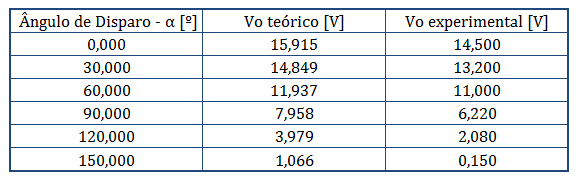
\includegraphics[keepaspectratio=true, scale=0.8]{teoricas/tabela1.png}
	\caption{Valores da tensão na carga teóricos e experimentais em função de $\alpha$}
	\label{fig:tabela1}
	\vspace{-0.8em}
\end{figure}

\begin{figure}[h]
	\centering
	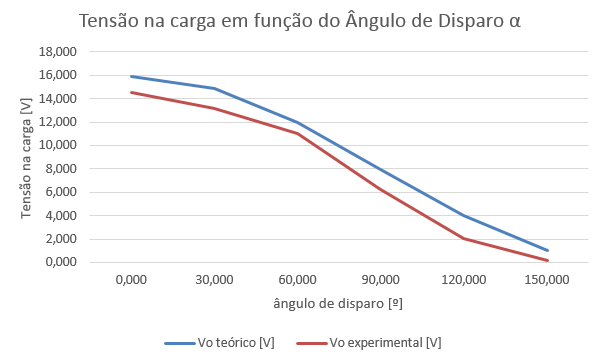
\includegraphics[keepaspectratio=true, scale=0.8]{teoricas/grafico1.png}
	\caption{Formas de onda da Tensão na carga teóricas e experimentais em função de $\alpha$}
	\label{fig:grafico1}
	\vspace{-0.8em}
\end{figure}


Verifica-se que existe pouca diferença entre os valores, podendo estas dever-se maioritariamente com o facto de para os cálculos teóricos se considerar que todos os dispositivos são ideais, o que não é válido na realidade.

\subsubsection{Carga indutiva RL}

Para estudar o comportamento de um retificador de meia onda com uma carga indutiva introduziu-se uma bobina em série com o reóstato.

\paragraph{Formas de onda da tensão e corrente na saída}

\todo{inserir imagem Carga Indutiva}

Na \textcolor{red}{Figura Carga Indutiva} podem ser observadas as formas de onda da tensão (a amarelo) na entrada do retificador e a tensão (a azul) e corrente (a rosa) na carga.

Ao contrário do que se tinha no caso da carga resistiva observa-se que a tensão na carga irá apresentar valores negativos; isto deve-se a que o tiristor apenas deixa de conduzir quando a corrente for zero e como a bobina introduz uma diferença de fase entre tensão e corrente pode observar-se valores de tensão negativos até que o dispositivo entre ao corte.

\paragraph{Formas de onda da tensão e corrente no tiristor}


\todo{não temos as imagens para esta parte nem valores para fazer as contas. faço a mesma sugestão que ja tinha feito, imagens da simulação. falta também fazer as contas dificeis!}

\subsubsection{Carga indutiva RL e díodo de roda livre}

Por fim, introduz-se no retificador um díodo de roda livre em antiparalelo com a carga para se estudar o seu impacto no circuito.

Teoricamente a introdução deste díodo deverá garantir que a tensão na carga não passará de zero devido à adição de uma indutância, pelas razões comentadas anteriormente.


\paragraph{Formas de onda da tensão e corrente na saída}

\todo{inserir imagem bobina com alfa diferente de zero}

Na \textcolor{red}{Figura bobina com alfa diferente de zero} tem-se a tensão na entrada do retificador (a amarelo) e tensão (a azul) e corrente (a rosa) na carga.

Observa-se que existe um ligeiro intervalo no qual a tensão na carga ainda é menor que zero, embora um valor muito inferior ao que se tinha no caso da carga RL sem díodo de roda livre. Isto deve-se a que nesse período a tensão observável será igual à de polarização direta do díodo de roda livre, que como está em antiparalelo com a carga, entra em condução na alternância negativa da tensão. 

\paragraph{Formas de onda da tensão e corrente no tiristor}

\todo{inserir imagem tiristor com alfa zero}

\todo{inserir imagem tiristor com alfa diferente de zero}

Na \textcolor{red}{Figura tiristor com alfa zero} tem-se a tensão na entrada do retificador (a amarelo) e corrente (a rosa) no tiristor, para $\alpha = 0$, sendo o comportamento para $\alpha$ diferente de $0$ observável na \textcolor{red}{Figura tiristor com alfa diferente de zero}.

Nestas figuras no entanto não se observa a tensão aos terminais do tiristor (a azul tem-se sim a tensão na carga). O comportamento expectável para esta seria apresentar o valor de tensão de polarização direta enquanto o dispositivo está à condução e a tensão na entrada do retificador enquanto está ao corte.

\paragraph{Formas de onda da tensão e corrente no díodo e na bobina}

\todo{inserir imagem diodo com alfa zero}

\todo{inserir imagem diodo com alfa diferente de zero}

Na \textcolor{red}{Figura diodo com alfa zero} tem-se a tensão na entrada do retificador (a amarelo), a tensão na carga (a azul) e corrente no diodo de roda livre (a rosa) para $\alpha = 0$. Já a \textcolor{red}{Figura diodo com alfa diferente de zero} tem-se o comportamento para $\alpha$ diferente de $0$.

Nota-se que a corrente que percorre o díodo é zero até ao momento em que a tensão na carga toma valores negativos. Nesse instante o díodo fica diretamente polarizado e a corrente observável é a de descarga da bobina, que irá decair de forma exponencial até $0$.

\todo{inserir imagem bobina com alfa zero}

Na \textcolor{red}{Figura bobina com alfa zero} tem-se a tensão na entrada do retificador (a amarelo), a tensão na carga (a azul) e corrente na bobina (a rosa) para $\alpha = 0$. Na \textcolor{red}{Figura bobina com alfa diferente de zero} tem-se o comportamento para $\alpha$ diferente de $0$.

Nota-se que embora a tensão na bobina não tenha sido lida, o seu comportamento é conhecido, devendo ter uma forma tal que o seu valor médio seja nulo. Já a corrente comporta-se tal como para o caso de uma carga indutiva até ao momento em que o díodo entra em condução. Nesse instante a corrente apresenta um comportamento exponencial decrescente; isto é similar ao comportamento da corrente que percorre o díodo de roda livre no mesmo período.

Conhecendo agora o comportamento do circuito observa-se que existem duas fases de funcionamento distintas.

Na primeira tem-se alternância positiva da tensão; o tiristor está diretamente polarizado e conduz assim que haja sinal de disparo, o díodo está inversamente polarizado e a tensão na carga é tal como a de entrada.

A segunda fase corresponde à alternância negativa da tensão de entrada; o díodo de roda livre está diretamente polarizado, sendo percorrido pela corrente da carga, passando ao corte assim que a bobina fique descarregada. Já o tiristor está inversamente polarizado, ficando ao corte assim que a corrente passe por zero

\section{Simulação do Trabalho de Laboratório}

\todo{this is our expertise teddy}

\subsection{Circuito de disparo}

\subsection{Circuito de potência}

\pagebreak

\begin{thebibliography}{2}
	
	\bibitem{Kassakian}
	Kassakian, John G. et al (1992, June), Principles of Power Electronics, \textit{Addison-Wesley Publishing Company}

	\bibitem{Rashid}
	Rashid, Muahammad H. (2004), Power Electronics - Circuits, Devices and Applications, \textit{Prentice Hall}
	
	\bibitem{Silva}
	Silva, Fernando (1998), Eletrónica Industrial, Fundação Calouste Gulbenkian
	
\end{thebibliography}


\pagebreak



\end{document}
